\documentclass{scrartcl}
\usepackage[utf8]{inputenc}
\usepackage{bussproofs}
\usepackage{scrpage2}
\usepackage{rotating}
\usepackage{listings}
\usepackage{amsmath}
\usepackage{amsfonts}
%\usepackage{mathtools}
\usepackage{hyperref}
\pagestyle{scrheadings}
\renewcommand{\thesubsection}{\alph{subsection}}
\clearscrheadfoot
\ohead[]{Nikolas Zeitler, Joshua Hartmann, Alexander Diegel}
\cfoot[\pagemark]{\pagemark}
\author{Nikolas Zeitler, Joshua Hartmann, Alexander Diegel}
\title{Maschinelles Lernen Blatt 2}

\begin{document}
\maketitle 
%Piss einfaches LatexFile für hausaufgaben, sieht nicht so hübsch aus aber es ist ausreichend
\section{Fragen zur Vorlesung}
\subsection{Wie lautet der Satz von Bayes? Welche Anwendungen dieses Satzes wurden in der Vorlesung vorgestellt?}
Der Satz lautet: \[P(X|Y) = \frac{P(Y|X)P(X)}{P(Y)} \] \\
Anwendungen des Satzes waren unter anderem das Ziegenproblem oder der Münzwurf, bei dem bestimmt werden sollte ob die Münze in Ordnung war oder nicht (Parameterschätzung).
In der Vorlesung haben wir das Bayes Theorem für "Parameterschätzung" verwendet. \\
\paragraph{Parameterschätzung:} Prüfen einer Hypothese anhand von bekannten Daten (a posteriori). Hier berechnet man beispielsweise die Wahrscheinlichkeitsdichtefunktion einer Münze, wenn man herausfinden möchte ob diese fair ist oder nicht anhand des Satzes von Bayes (vgl. Skriptum S.32).
\\ (ist wenn man aus gegebenen Daten die \textit{likelihood} von parametern dieser Daten bestimmen will. )
(@Team puuh k.a. Script S 11.)

\subsection{Wie kann man den Satz von Bayes in Bezug auf eine Hypothese interpretieren, die man auf der Basis von ermittelten Daten prüfen möchte?}
Die Festlegung wie glaubhaft die ermittelten Daten sind und wie glaubhaft die Hypothese ist legt fest, wie glaubhaft die Hypothese unter den gegebenen Daten ist. (Glaubhaftigkeit der Hypothese auf Basis der gegebenen Daten.)
Bayes kann bei einer Hypothese dabei helfen zu wie groß die Wahrscheinlichkeit ist, das diese korrekt bzw falsch ist. 
(@Team yoah ich weis nciht was der noch will???)


\subsection{Die (absolute) Wahrscheinlichkeit, dass die gegebenen Daten vorliegen, (auch bezeichnet als evidence) ist unabhängig von der Hypothese. Im Satz von Bayes ist daher (Foliensatz 2, Folie 24) der Nenner bei der Hypothesenbewertung in gewisser Hinsicht qualitativ vernachlässigbar. Wann ist er dennoch wichtig? Fasst kurz zusammen, in welchen Fällen die evidence vernachlässigt werden kann und in welchen nicht.}
Für das Beispiel aus dem Script gilt: 
%\\ich mach das mal raus, weiß nicht ob das so relevant ist, ich glaub der Punkt ist das P(Daten) fest ist
%\[P(Daten) = \sigma P(Daten|Hypothese)P(Hypothese) \]@TEAM WARUM SIGMA? 
%>>$P(Daten)=P(Daten|Hypothese)P(Hypothese)+P(Daten|\neg Hypothese)P(\neg Hypothese)=1$
%In Fällen in denen $\sigma P(Daten|Hypothese)P(Hypothese)=1$ kann auf ihn verzichtet werden. Da dann %$\frac{P(Daten|Hypothese)P(Hypothese)}{1}$\\

Es kann vernachlässigt werden wenn die evidence ($P(Daten)$) "fixed" ist und wir den Parameter "Hypothese" variieren möchten. Beispielsweise beim Münzwurf ist die Wk für Kopf immer 0.5 (vereinfacht) und kann deswegen ignoriert werden. Auch  bei der Anwendung der Entscheidungsregel kann die Evidence vernachlässigt werden (Skriptum S. 40).\\
Beispiel:\\Bei Versuchen in denen die P(daten) variieren können, Bspw. bei Messungen mit einem Lasersensor zu Erstellung einer occupancy map. Können andere Fehler auftreten. \\
(@Team. da bin ich mir jetzt doch sehr unsicher -- denke das Beispiel ist ok) 

\subsection{Wie kann man zwischen zwei Hypothesen $\omega_1$ und $\omega_2$ entscheiden, wenn keine Daten vorliegen? ($P(\omega_i), i=1,2$ darf dabei als bekannt vorausgesetzt werden.)}
Mit der Entscheidungsregel (Klassifikation) (Folie S.35) \\
$\omega_1, wenn P(\omega_1 ) > P(\omega_2) $ \\
$\omega_2 sonst.$\\
Hierfür benötigt man nur die gegebenen A-priori Wahrschenlichkeit. \\

\subsection{Warum summieren sich auf Folie 38 (Foliensatz 2) die Funktionswerte punktweise (d. h. für jedes einzelne x) genau zu 1 und auf Folie 36 nicht? Sind die entsprechenden Integrale über den Wertebereich von x jeweils 1?(Überlegt dazu genau, was die Grafiken zeigen.)}

Seite 38 sieht man die a-Posteriori Wahrscheinlichkeiten, hier muss die summierte Wahrscheinlichkeit für jedes x 1 ergeben, da entweder $\omega_1$ oder $\omega_2$ richtig ist und es keine andere Möglichkeit gibt. Das Integral muss nicht 1 sein, da es sich nicht um eine Wahrscheinlichkeitsdichte handelt.\\
Auf Seite 36 werden verschiedene Wahrscheinlichkeitsdichten angezeigt, für jede einzelne ist das Integral also 1. Da es sich um Wahrscheinlichkeitsdichten handelt gelten keine besonderen Regeln, was einzelne Funktionswerte angeht, insbesondere addieren sich die beiden Kurven also nicht zu 1.

\subsection{Erkläre, was die Bayes’sche Entscheidungsregel besagt. (Siehe dazu Foliensatz 2, Folie 39 oder Duda S. 42.)}
Mit der Entscheidungsregel kann man sich für die Hypothese entscheiden, mit welcher man das Gesamtrisiko minimiert. Das führt zu einer optimalen Entscheidungsregel. 

\subsection{Welches Risiko drückt das (conditional) risk aus? (Dieses findet sich in Foliensatz 2 auf S. 41; siehe auch Duda S. 43 / 44.)}
Das Risiko drückt aus, wie "teuer" eine Fehleinschätzung zu einer Hypothese anhand der Daten ist. (Beispiel: Wir entscheiden uns bei einer Länge x für Barsch, obwohl es ein Lachs war). 


\subsection{Wie hängen das sogenannte Bayes risk (Foliensatz 2, Folie 43 bzw. Duda S. 44) und das Gesamtrisiko (Foliensatz 2, Folie 42) zusammen?}
Das Bayesrisiko ist das kleinst mögliche Gesamtrisiko welches erreicht werden kann (optimale Entscheidungsregel). \\
Das Gesamtrisiko ist der Erwartungswert der Fehler/das mittlere Risiko, die bei der Schätzung gemacht werden. (Integral/Fläche unter der Risikofunktion).

\section{Bayes'scher Fisch-Klassifikator}

\subsection{Einlesen der Daten} 
\subsection{Histogramm der Daten}
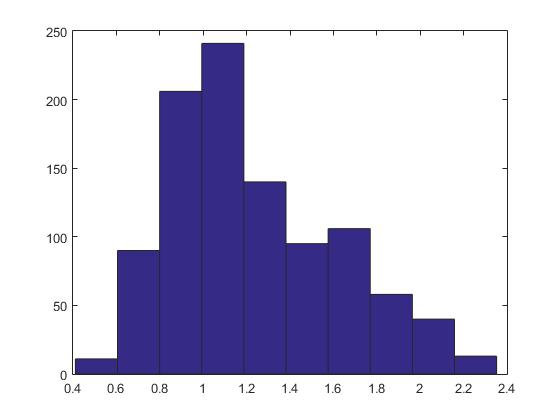
\includegraphics[width=.6\textwidth]{plots/2b_hist.jpg}

\subsection{Anwendung des Satz von Bayes}
Siehe Matlab-File

\subsection{Plot für die bedingten Funktionen $\mathbb{P}(\omega_j|x)$, j=1,2}
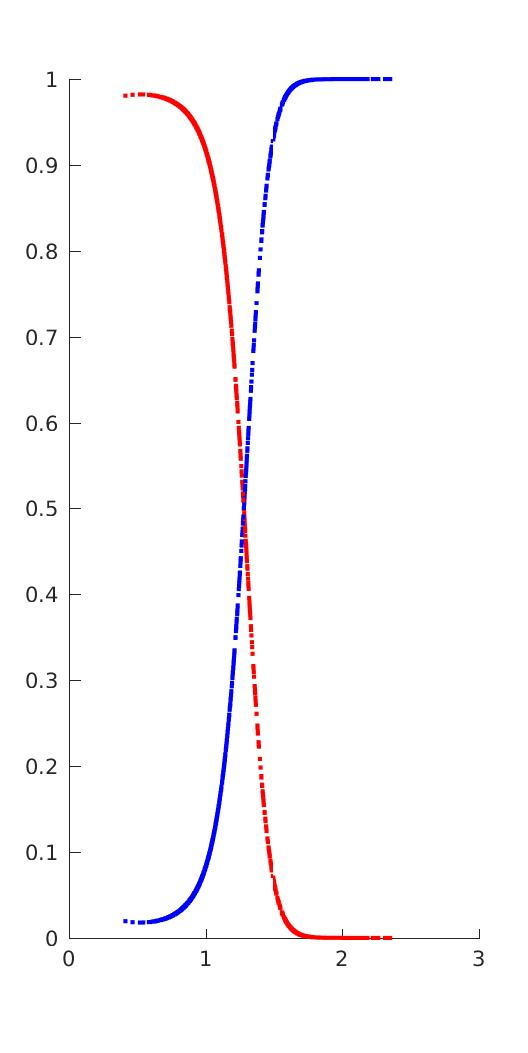
\includegraphics[width=.6\textwidth]{plots/2d_bedingte_wk.jpg}\\
rot: Barsch, blau: Lachs

\subsection{Anwenden der Bayes'schen Entscheidungregel}
Siehe Matlab-File.

\subsection{Wahrscheinlichkeit für das Vorliegen eines Barsches oder Lachses}

Lachs: 0.378\\
Barsch: 0.622

\subsection{Inwiefern ist das Klassifikationsverfahren abhängig von den Annahmen?}
 Die Klassifikation ist abhängig von den Annahmen über die relative Anzahl der Fische und der gewählten Verteilungen der Fischlängen.
 
\section{Loss-Funktion, Risiko}
\subsection{Risiko für irrtümliche Entscheidung}
Siehe Matlab-File

\subsection{Plot des conditional risks für Barsche und Lachse}

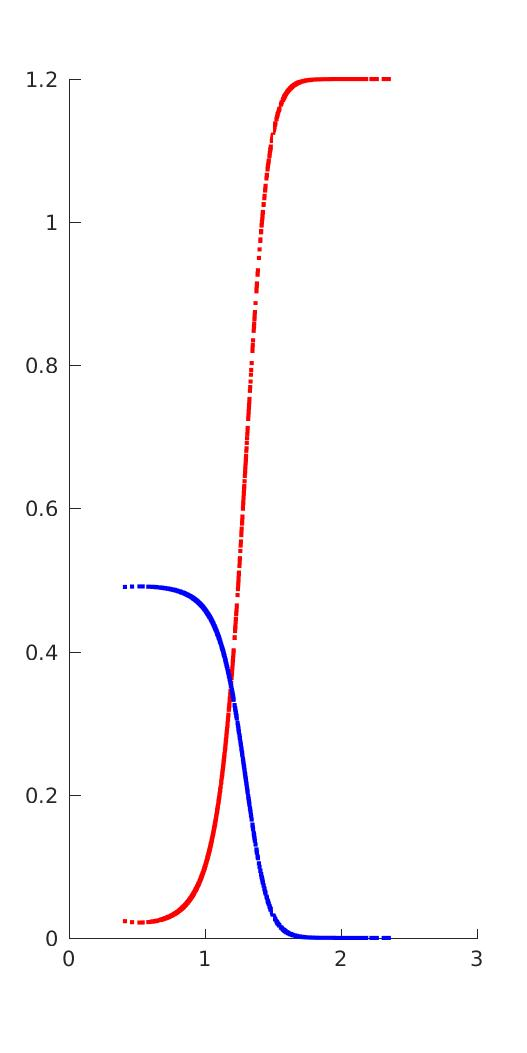
\includegraphics[width=.6\textwidth]{plots/3b_conditional_risk.jpg}\\
rot: Barsch, blau: Lachs
\subsection{Klassifikation anhand des conditional risk}
Siehe Matlab-File.

Ergebnis: 550 Barsche, 450 Lachse

\subsection{Abgeänderte Loss Funktion}
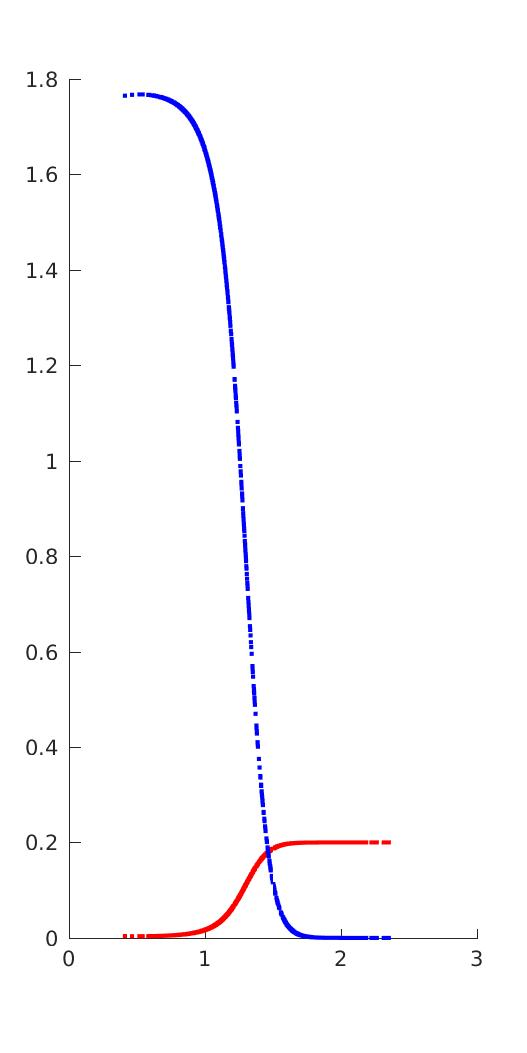
\includegraphics[width=.6\textwidth]{plots/3d_conditional_risk.jpg}\\
rot: Barsch, blau: Lachs\\

Es ist 'teurer' geworden, einen Fisch als Lachs zu klassifizieren, obwohl es ein Barsch war. Daher entscheiden wir uns jetzt häufiger dafür, dass es sich um einen Barsch handelt als vorher.
\end{document}